\subsection{Programme)
	Programme of autonomous period (algorithm):
	\begin{enumerate}
		\item Move forward by encoders.
		
		\item Do tank turning with help of compass sensor.
		
		\item Move forward by encoders.
		
		\item Tank turn with compass.
		
		\item Move forward to shelter.
		
		\item Turn servo on mechanism for scoring climbers and put them to shelter.
		
		\item Stay in repair zone.
		
		%\begin{figure}[H]
		%	\begin{minipage}[h]{1\linewidth}
		%		\center{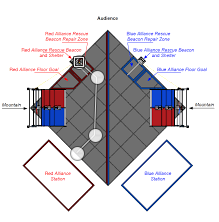
\includegraphics[scale=0.5]{key_chapters/images/01}}
		%		\caption{Trajectory of robot during autonomous period}
		%	\end{minipage}
		%\end{figure}
	\end{enumerate}
	
	Operational Period
	\begin{itemize}
		\item During most of the local competitions we used the old NXT-based system, but closer to the regional finals in Sochi we finally got our kits and started working on installing the new systems. There were not many problems with installing the hardware itself, but the programming proved to be more challenging due to the new software, language, and tools. Nevertheless, we were able to create our programs in time for the regional finals.
	\end{itemize}
